\documentclass{article}
\usepackage{amsmath}
\usepackage{amssymb}
\usepackage{geometry}
\usepackage{graphicx}
\usepackage{setspace}
\usepackage{enumerate}
\usepackage[dvipsnames]{xcolor}
\geometry{a4paper, portrait, margin=.2in}

\title {EIND 464: Homework 5}
\date{4/5/2023}
\author{Thomas Lipinski}
\begin{document}
\maketitle
\onehalfspacing
\subsection*{Section 17.2} 
\begin{enumerate}
\item[3) ]\textbf{A company has two machines. During any day, each machine that is working at the beginning of the day has a $\frac{1}{3}$ chance of breaking down. If a machine breaks down during the day, it is sent to a repair facility and will be working two days after it breaks down. (Thus, if a machine breaks down during day 3, it will be working at the beginning of day 5.) Letting the state of the system be the number of machines working at the beginning of the day, formulate a transition probability matrix for this situation.}

States : [Both broken, one working, both working].\\
A breakdown takes the machine out of service for the remainder of the day + 1 day.\\
If both machines are down at the start of a day, they will both be online tomorrow. \\
If neither machine is down today, they both have a $\frac{1}{3}$ chance of breaking down. (2/3 chance one will go down, 1/9 chance both will go down)\\
If a machine is down, it will be back online tomorrow. 
\[
P = 
\begin{bmatrix}
0 & 0 & 1\\
0 & \frac{1}{3} & \frac{2}{3}\\
\frac{1}{9} & \frac{4}{9} & \frac{4}{9}
\end{bmatrix}\hspace*{1cm}
\]

\item[6) ] \textbf{In Problem 3, suppose a machine that breaks down returns to service three days later (for instance, a machine that breaks down during day 3 would be back in working order at the beginning of day 6). Determine a transition probability matrix for this situation.}\\
States : [zero working, one working, two working].

If both machines are working at the beginning of today, there is a $\frac{1}{3}\cdot\frac{1}{3}=\frac{1}{9}$ chance both fail. P(2,0) = $\frac{1}{9}$.\\
There is a $2\cdot(\frac{1}{3} - \frac{1}{9}) $ chance that one of the two machines fails P(2,1) = $\frac{4}{9}$\\
There is a $\left(\frac{1}{9}\right)^2 $ chance that neither of the two machines fails P(2,2) = $\frac{4}{9}$

If one machine is working at the start of the day, there is a 1/3 chance it fails for tomorrow. If the other machine failed two days ago, it will be back tomorrow, leading to states of \{0: 0, 1: $\frac{1}{3}$, 2: $\frac{1}{3}$\}. If the other machine failed yesterday, it will not be back tomorrow, leading to states of \{0:$\frac{1}{3}$, 1: $\frac{2}{3}$, 2: 0\}. taking the average of these states produces Row 2 = [$\frac{1}{6}$ $\frac{1}{2}$ $\frac{1}{3}$]

On to Row 1.... If neither machine is functional today, there are three ways this is possible:

Both machines failed two days ago (both will be online tomorrow).\\
One machine failed two days ago, the other machine failed yesterday (One machine will be online tomorrow).\\
Both machines failed yesterday (neither will be online tomorrow).\\
\emph{How to calculate the probability of starting in these states?}\\
Assuming that each of these states is equally likely to be started in, then each of these states has a $\frac{1}{3}$ chance of occurring,
\[
P = 
\begin{bmatrix}
\frac{1}{3} & \frac{1}{3} & \frac{1}{3}\\
\frac{1}{6} & \frac{1}{2} & \frac{1}{3}\\
\frac{1}{9} & \frac{4}{9} & \frac{4}{9}
\end{bmatrix}\hspace*{1cm}
\]

\end{enumerate}
\subsection*{Section 17.3}
\begin{enumerate}
\item[2) ]\textbf{The following questions refer to Example 1 (Gambler's Ruin)}
\begin{enumerate}
\item[a) ]\textbf{After playing the game twice, what is the probability that I will have \$3? How about \$2?}\\
	If the game is played once, the is p chance of having \$3 and (1-p) chance of having \$1. 
	if the game is played twice, there are four possible states (two are absorbing, (p)(p) = \$4 and (1-p)(1-p) = \$0). The non-absorbing states are (p)(1-p) = \$2, and (1-p)(p) = \$2.\\
\colorbox{Goldenrod}{P($X_2$ = 3) = 0 and P($X_2$ = 2) = 2$\cdot$(p)(1-p)}
	
\item[b) ]\textbf{After playing the game three times, what is the probability that I will have \$2?\\}
Building off part \emph{a}, the possible states at t = 2 are \$0, \$2, and \$4. There is no way to get to \$2 
from these states, so \colorbox{Goldenrod}{P($X_3$ = 2) = 0}
\end{enumerate}

\item[3) ] \textbf{In Example 2, determine the following n-step transition probabilities:}
\begin{enumerate}
\item[a) ]\textbf{After two balls are painted, what is the probability that the state is [0 2 0]?}

There are 6 states at t = 2, one of which is [0 2 0]. therefore, \colorbox{Goldenrod}{1/6}

\item[b) ]\textbf{After three balls are painted, what is the probability that the state is [0 1 1]? (Draw a diagram like Figure 4.)}

There are 12 states at t = 3, four of which are [0 1 1]. therefore, \colorbox{Goldenrod}{1/3}

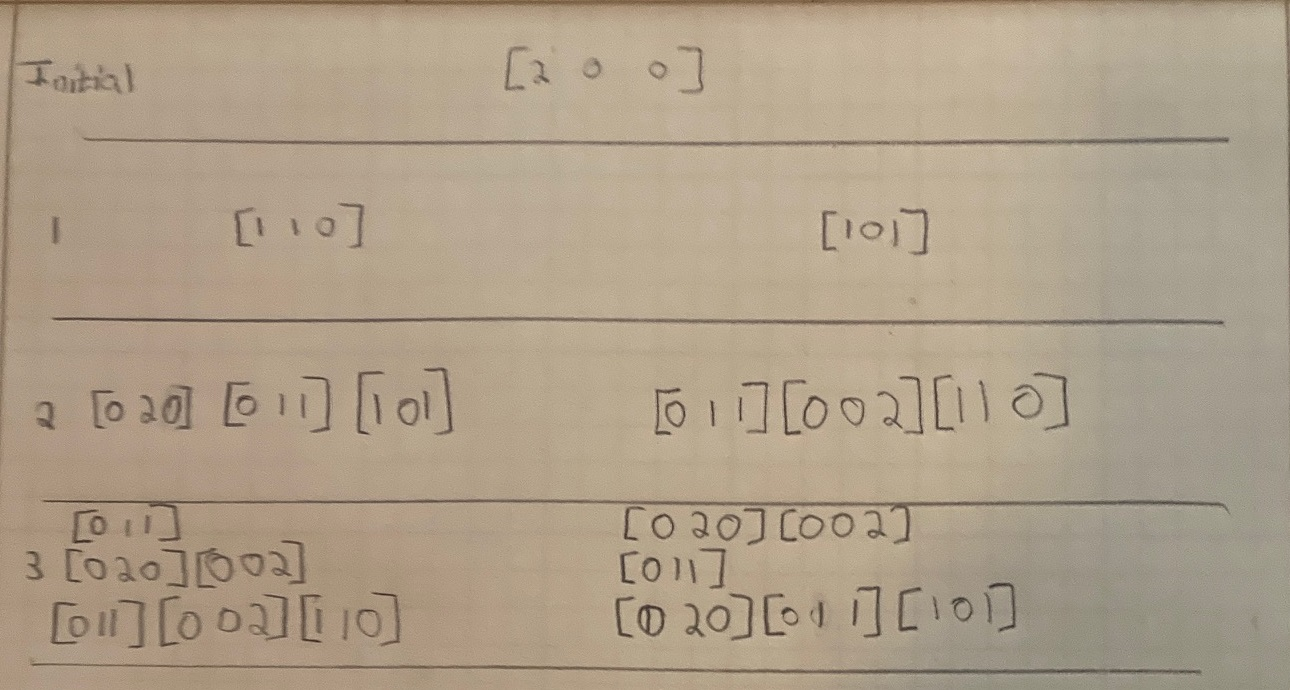
\includegraphics[scale=.44]{17_3.JPG}

\end{enumerate}

\end{enumerate}
\subsection*{Section 17.4}
\begin{enumerate}
\item[3) ] \textbf{Consider the following transition matrix:}
\[
P = 
\begin{bmatrix}
0 & 0 & 1 & 0 & 0 & 0\\
0 & 0 & 0 & 0 & 0 & 1\\
0 & 0 & 0 & 0 & 1 & 0\\
\frac{1}{4} & \frac{1}{4} & 0 & \frac{1}{2} & 0 & 0\\
1 & 0 & 0 & 0 & 0 & 0\\
0 & \frac{1}{3} & 0 & 0 & 0 & \frac{2}{3}
\end{bmatrix}
\]
In P: 1 can reach 3, 3 cannot reach 1. 

2 can reach 6, 6 can reach 2. 

3 can reach 5, 5 cannot reach 3. 

4 can reach 1 2, 1 and 2 cannot reach 4.

4 can reach 4. 

5 can reach 1, 1 cannot reach 5. 

6 can reach 6.  

\begin{enumerate}
\item[a) ] \textbf{Which states are transient?} State \colorbox{Goldenrod}{2} cannot reach itself.
\item[b) ] \textbf{Which states are recurrent?} States \colorbox{Goldenrod}{1 3 4 5 6} can reach themselves.
\item[c) ] \textbf{Identify all closed sets of states.} \colorbox{Goldenrod}{S = \{2 4 6\}}
\item[d) ] \textbf{Is this chain ergodic?} \colorbox{Goldenrod}{No, not all nodes communicate.}

\end{enumerate}
\item[5) ] \textbf{Fifty-four players (including Gabe Kaplan and James Garner) participated in the 1980 World Series of Poker. Each player began with \$10,000. Play continued until one player had won everybody else’s money. If the World Series of Poker were to be modeled as a Markov chain, how many absorbing states would the chain have?}

\colorbox{Goldenrod}{There would be 54 absorbing states--one for each player taking all the money from their opponents.}

\end{enumerate}
\subsection*{Section 17.5}
\begin{enumerate}
\item[7) ] \textbf{Consider two stocks. Stock 1 always sells for \$10 or \$20. If stock 1 is selling for \$10 today, there is a .80 chance that it will sell for \$10 tomorrow. If it is selling for \$20 today, there is a 90\% chance that it will sell for \$20 tomorrow. Stock 2 always sells for \$10 or \$25. If stock 2 sells today for \$10, there is a 90\% chance that it will sell tomorrow for
\$10. If it sells today for \$25, there is a 85\% chance that it will sell tomorrow for \$25. On the average, which stock will sell for a higher price? Find and interpret all mean first passage times.}

\[
s_1 = 
\begin{bmatrix}
.8 & .2\\
.1 & .9 
\end{bmatrix}\hspace*{2mm}\rightarrow\hspace*{2mm}
s_1^{50000} = 
\begin{bmatrix}
\frac{1}{3} & \frac{2}{3}\\
\frac{1}{3} & \frac{2}{3} 
\end{bmatrix}\hspace*{1cm}
s_2 = 
\begin{bmatrix}
.9 & .1\\
.15 & .85 
\end{bmatrix}\hspace*{2mm}\rightarrow\hspace*{2mm}
s_2^{50000} = 
\begin{bmatrix}
.6 & .4\\
.6 & .4
\end{bmatrix}
\]
Now that SSPTMs have been calculated, multiply SSPTM by the value vector [10 20] for $S_1$, and [10 25] for $S_2$. This gives an expected sale value of \$16.67 for stock 1, and \$16.00 for stock 2. \colorbox{Goldenrod}{Stock 1 sells for $2/3^{rds}$ of a dollar more. }

Calculate Mean passage times, held in matrix M. $M_{ii} = \frac{1}{\pi_i}$, so diagonals are done. The off diagonals can be computed with $M_{ij} - P_{ii}M_{ij} = 1$. 
\[
M_1 = 
\begin{bmatrix}
3 & 5\\
10 & \frac{3}{2} 
\end{bmatrix}\hspace*{1cm}
M_2 = 
\begin{bmatrix}
\frac{5}{3} & 10\\
\frac{20}{3} & \frac{5}{2}
\end{bmatrix}
\]

\colorbox{Goldenrod}{It is twice as common for $M_{12}$ in stock 1 vs stock 2, meaning the earnings are at their high state more often. }

\colorbox{Goldenrod}{They also get demoted $M_{21}$ at at only 2/3rds the rate in stock 1. Stock 1 has a faster cycle times and spends}

\colorbox{Goldenrod}{more time in high earning states.}

\item[13) ] \textbf{An important machine is known to never last more than four months. During its first month of operation, it fails 10\% of the time. If the machine completes its first month, then it fails during its second month 20\% of the time. If the machine completes its second month of operation, then it will fail during its third month 50\% of the time. If  machine completes its third month, then it is sure to fail by the end of the fourth month. At the beginning of each month, we must decide whether or not to replace our machine with a new machine. It costs \$500 to purchase a new machine, but if a machine fails during a month, we incur a cost of \$1,000 (due to factory downtime) and must replace the machine (at the beginning of the next month) with a new machine. Three maintenance policies are under consideration:}

\begin{enumerate}
\item[\textbf{1}] Plan to replace a machine at the beginning of its fourth month of operation.
\item[\textbf{2}] Plan to replace a machine at the beginning of its third month of operation.
\item[\textbf{3}] Plan to replace a machine at the beginning of its second month of operation.
\end{enumerate}

\textbf{Which policy will give the lowest average monthly cost?}
\[
P = 
\begin{bmatrix}
.1 & .9 & 0 & 0\\
.2 & 0 & .8 & 0\\
.5 & 0 & 0 & .5\\
1 & 0 & 0 & 0
\end{bmatrix}
\]
$\vec{\pi} = \begin{bmatrix} \pi_1 & \pi_2 & \pi_3 & \pi_4 \end{bmatrix}$, And we know $\Sigma \vec{\pi} = 1. $ Need to find the steady state probability matrix.
\begin{align}
  0.1\pi_1 + 0.2\pi_2 + 0.5\pi_3 + \pi_4 &= \pi_1 \nonumber \\
  0.9\pi_1 &= \pi_2 \nonumber \\
  0.8\pi_2 &= \pi_3 \nonumber \\
  0.5\pi_3 &= \pi_4 \nonumber
\end{align}
The first equation is busy. Swapping it out for $\pi_1 + \pi_2 + \pi_3 + \pi_4 = 1$\\
Solved the linear equations with a calculator; $\pi_1 = 0.33557$, $\pi_2 = 0.30213$, $\pi_3 = 0.241611$, $\pi_4 = 0.120805$.

Now for finding average monthly costs...  \emph{failed to replicate this with the steady-state matrix.}
\begin{align}
  PS_1 \cdot 1000 + PF_1 \cdot 500 = c_1 = 0.1 \cdot 1000 + 0.9  \cdot  500 = 550 \nonumber \\
  PS_2 \cdot 1000 + PF_2 \cdot c_1 = c_2 = 0.2 \cdot 1000 + 0.8 \cdot 550 = 620 \nonumber \\
  PS_3 \cdot 1000 + PF_3 \cdot c_2 = c_3 = 0.5 \cdot 1000 + 0.5 \cdot 500 = 820 \nonumber \\
  \colorbox{Goldenrod}{Policy 1 is the best with an average monthly cost of \$550 \nonumber.}\\
  \text{I ran a Monte-Carlo simulation to find the answer and worked backwards to it...}\nonumber
\end{align}
\end{enumerate}
\subsection*{Section 17.6}
\begin{enumerate}
\item[5) ] \textbf{Each week, the number of acceptable-quality units of a drug that are processed by a machine is observed: \\$\left[>100, 50–100, 1–50, 0\right]$ (indicating that the machine was broken during the week). Given last week’s observation, the probability distribution of next week’s observation is as follows}
\[
\begin{bmatrix}
>100\\
50-100\\
1-50\\
0
\end{bmatrix}
\begin{bmatrix}
.8 & .1 & .05 & .05\\
.1 & .6 & .1 & .2\\
.1 & .1 & .5 & .3\\
0 & 0 & 0 & 1
\end{bmatrix}
\]
\textbf{For example, if we observe a week in which more than 100 units are produced, then there is a .10 chance that during the next week 50–100 units are produced.}
\begin{enumerate}
\item[a) ] \textbf{Suppose last week the machine produced 200 units. On average, how many weeks will elapse before the machine breaks down?}


$\vec{\pi}$ = [9.32203,  6.10169,  5.08475,  0] 

\colorbox{Goldenrod}{9.322 weeks}


\item[b) ] \textbf{Suppose last week the machine produced 50 units. On average, how many weeks will elapse before the machine breaks
down?}
\colorbox{Goldenrod}{6.102 weeks}


\end{enumerate}

\item[11) ] \textbf{Freezco, Inc., sells refrigerators. The company has issued a warranty on all refrigerators that requires free replacement of any refrigerator that fails before it is three years old. We are given the following information: (1) 3\% of all new refrigerators fail during their first year of operation; (2) 5\% of all one-year-old refrigerators fail during their second year of operation; and (3) 7\% of all two-year-old refrigerators fail during their third year of operation. A replacement refrigerator is not covered by the warranty.}
\begin{enumerate}
\item[a) ] \textbf{Use Markov chain theory to predict the fraction of all refrigerators that Freezco will have to replace.}

\[
(I - Q)' \cdot R = 
\begin{bmatrix}
 -0.121104  &   0.0780713&  -2.05813\\
  0.0860233   & 1.3928   &   0.591191\\
  2.02292e-17 & 0.745299  & -0.448101\\
  \end{bmatrix}\\
\]
\text{sum of} $(I - Q)' \cdot R $ = \colorbox{Goldenrod}{0.2661}\\
This is wrong as I am not accounting for the replacement fridges not being valid for replacement. I am tired and need to go to bed for our 2nd exam tomorrow. This will do I hope.

\item[b) ] \textbf{Suppose that it costs Freezco \$500 to replace a refrigerator and that Freezco sells 10,000 refrigerators per year. If the company reduced the warranty period to two years, how much money in replacement costs would be saved?}


\colorbox{Goldenrod}{1 million dollars}

\end{enumerate}
\end{enumerate}


\end{document}